%% Template for Master thesis
%% ===========================
%%
%% You need at least KomaScript v3.0.0,
%% e.g. available in Texlive 2009
\documentclass  [
  paper    = a4,
  BCOR     = 10mm,
  twoside,
  fontsize = 12pt,
  fleqn,
  toc      = bibnumbered,
  toc      = listofnumbered,
  numbers  = noendperiod,
  headings = normal,
  listof   = leveldown,
  version  = 3.03
]                                       {scrreprt}

% used pagages
\usepackage     [utf8]                  {inputenc}
\usepackage     [T1]                    {fontenc}
\usepackage                             {color}
\usepackage                             {amsmath}
\usepackage                             {graphicx}
\usepackage								{epsfig}
\usepackage     [english]               {babel}
\usepackage                             {natbib}
\usepackage                             {hyperref}
\usepackage								{amssymb}
%\usepackage{BibLatex}
% links
\definecolor{darkblue}{rgb}{0.0,0.0,0.4}
\definecolor{darkgreen}{rgb}{0.0,0.4,0.0}
\hypersetup{
    colorlinks,
    linkcolor=black,
    citecolor=darkgreen,
    urlcolor=darkblue
}

\DeclareMathOperator*{\argmax}{argmax}

\begin{document}
  %% title pages similar to providet template instead of maketitle
  %% Titelseiten ähnlich zum Layout des Formulars von der
%% Fakultät für Physik und Astronomie
%%
%% Weitere Infos:
%% http://www.physik.uni-heidelberg.de/aktuelles/studium/
%% (PDF link: ...studium/download/145/Vorlage_Diplomarbeit_Formular.pdf)

%% Titelintro
\thispagestyle{empty}
\begin{center}
  \renewcommand{\baselinestretch}{2.00}
  \Large\sffamily
  Fakult\"{a}t f\"{u}r Physik und Astronomie\\
  \large
  Ruprecht-Karls-Universit\"{a}t Heidelberg
  \par\vfill\normalfont
  Masterarbeit\\
  Im Studiengang Physik\\
  vorgelegt von\\
  (Vor- und Zuname)\\
  geboren in (Geburtsort)\\
  (Jahr der Abgabe)\\
\end{center}
\newpage

%% Titelseite
\thispagestyle{empty}
\begin{center}
  \renewcommand{\baselinestretch}{2.00}
  \Large\bfseries\sffamily
    (Titel)\\
    (der)\\
    (Masterarbeit)
  \par
  \vfill
  \large\normalfont
  Die Masterarbeit wurde von (Vorname Name)\\
  ausgef\"{u}hrt am\\
  (Institut)\\
  unter der Betreuung von\\
  (Frau/Herrn Prof./Priv.-Doz. Vorname Name)
  %% Bei externen Masterarbeiten hier noch den zweiten Betreuer einfügen
  %% und den vspace in Z. 45 entsprechend reduzieren
\end{center}\par
\vspace{5\baselineskip}

% Zeilenabstand zurücksetzen
\renewcommand{\baselinestretch}{1.00}\normalsize % select either german
  %% this will generate title pages similar to the template provided
%% by the Department of Physics and Astronomy Heidelberg
%%
%% More information:
%% http://www.physik.uni-heidelberg.de/aktuelles/studium/
%% (PDF link: ...studium/download/145/Vorlage_Diplomarbeit_Formular.pdf)

%% Titleintro
\thispagestyle{empty}
\begin{center}
  \renewcommand{\baselinestretch}{2.00}
  \Large\sffamily
  Department of Physics and Astronomy\\
  \large University of Heidelberg
  \par\vfill\normalfont
  Master thesis\\
  in Physics\\
  submitted by\\
  Jacob Nieswand\\
  born in Konstanz\\
  2018
\end{center}
\newpage

%% Titlepage
\thispagestyle{empty}
\begin{center}
  \renewcommand{\baselinestretch}{2.00}
  \Large\bfseries\sffamily
    Optimizations of Light Field measurements\\
    using the structure tensor
  \par
  \vfill
  \large\normalfont
  This Master thesis has been carried out by Jacob Nieswand\\
  at the\\
  Institut für wissenschaftliches Rechnen (IWR)\\
  under the supervision of\\
  Herrn Priv.-Doz. Christoph Garbe
  %% additionally insert second supervisor here if carrying out an
  %% external diploma thesis. Reduce vspace in L. 44 accordingly.
\end{center}\par
\vspace{5\baselineskip}

% reset baselinestretch
\renewcommand{\baselinestretch}{1.00}\normalsize % or english title page
  %% Abstract page
%% =============
%%
%% Content of abstract pages has been put into seperate pages to simplify
%% word counting. Use e.g. the unix command
%%   wc abstract-ger.tex
%% or
%%   wc abstract-eng.tex
%% to get the number of words contained in these files.
\thispagestyle{empty}
\begin{center}
  \begin{minipage}[c][0.48\textheight][b]{0.9\textwidth}
    \small
    \textbf{
      Optimierung von EPI-basierten Lichtfeldmessungen:
    }\par
    \vspace{\baselineskip}
    
Diese Arbeit befasst sich mit der Tiefenrekonstruktion einer Szene mittels 2D-Aufnahmen aus verschiedenen Blickwinkeln (Lichtfeld). Aus der Struktur der epipolaren Schnitte durch das Lichtfeld (EPIs) wird mithilfe des Strukturtensors die Tiefe errechnet. In dieser Arbeit werden verschiedene Modifikationen bestehender entwickelter Algorithmen getestet, weiterhin werden Depth-of-defocus- Techniken getestet und verglichen. Zusätzlich wird ein Algorithmus basierend auf dem in der Stereo-Vision verbreiteten Semi-global Matching Algorithmus (SGM) als Nachbearbeitungsschritt implementiert.
  \end{minipage}\par
  \vfill
  \begin{minipage}[c][0.48\textheight][b]{0.9\textwidth}
    \small
    \textbf{
      (Title of Master thesis - english):
    }\par
    \vspace{\baselineskip}
    This work deas with 3D depth reconstruction of a scene using 2D images captured from different angles (light field imaging). From the structure of the Epipolar Plane Images (EPIs) the depth is calculated using the structure tensor In this thesis various modifications of existing algorithms will be developed and tested, further depth-of-defocus techniques will be tested and compared. In addition, an algorithm based on the SemiGlobal Matching Algorithm (SGM) ,commonly used in Stereo vision, is implemented as a postprocessing step.
  \end{minipage}
\end{center}


  \tableofcontents
  %% Put your contents here
\chapter{Theory}
\section{Light Field Parametrization}
The earliest introduction to Light Fields in literature can be found in \cite{adelson1991plenoptic}, where they parametrize the field of light as a  so-called \glqq plenoptic function \grqq. If we assume that every point in space emits a light ray  in a given direction which is characterized by a intensity value $P$, the whole information in the light field is given as a 5-dimensional function
\begin{equation}\label{key}
P(V_x,V_y, V_z, \theta, \phi, \lambda),
\end{equation}
where $\theta$ and $\phi$ are the solid angles describing the direction of any light field, $\lambda$ describes the wavelength dependence. $V_\{x,y,z\}$ describe the room coordinates. If we use the pixel of a pinhole camera picture as the coordinate system of our choice, the plenoptic function would be parametrized as 
\begin{equation}\label{eq:plenoptic}
P(x,y, V_x, V_y, V_z, \lambda).
\end{equation}
 A more generalized model of the plenoptic function could also include a time dependence, leading to a 7-dimensional ray space. In general, the plenoptic function serves as the global funcion that gets mapped into a low-dimensonal space in some form by any camera device, e.g. a pinhole camera mapping the whole ray space down to a 2-dimensional image.\\
 \setcitestyle{numbers}
 	
 A more detailed introduction to Lightfields can also be found in \cite{wanner2014orientation}. 
 \setcitestyle{authoryear}
\subsection{The Lumigraph}
In the form of \ref{eq:plenoptic} the plenoptic function is a 7-dimensional function, which is difficult to record and to handle. As described by \cite{wu2017light} this plenoptic function is usually simplified in 3 steps: First, we neglect the time dependence (assuming a static scene), further we neglect the wavelength $\lambda$, instead we define the mapped value of the plenoptic function as a vector containing the color channels. 
Additionally the plenoptic function obtains redundant information due to the fact, that light rays that are lying on one line in space propagate in the same direction, as introduced by \cite{bolles1987epipolar}. The 4D- representation is also known as the \textit{Lumigraph}. Those 4 dimensions can be split to 2 angular dimensions describing the direction of each ray and 2 dimensions for the loaction of the ray: Since every ray would pass an image plane of infinite size once (if the propagation vector is not parallel), two coordinates for localizing the ray are sufficient. Commonly the \textit{two-plane-parametrisation} is used to describe the light field. Every ray is characterized by the intersection of two arbitrary parallel planes $\Pi$ and $\Omega$. Mathematically spoken the light field $L$ is a function
\begin{equation}\label{key}
L:\Omega\times \Pi \rightarrow \!R\qquad x,y,s,t\rightarrow L(x,y,s,t),
\end{equation}
where $x,y$ are the coordinates in the first plane $\Omega$ and $s,t$ are the coordinates in the second plane $\Pi$. If we move a camera in a plane and take pictures of a scene orthogonal to the camera plane, the image itself is described by the image coordinates $x,y$ while the position of the camera is denoted as $s,t$. Both planes are parallel to each other; that way a light field can be measured in a straight forward manner.
\begin{figure}[h]
	\centering
	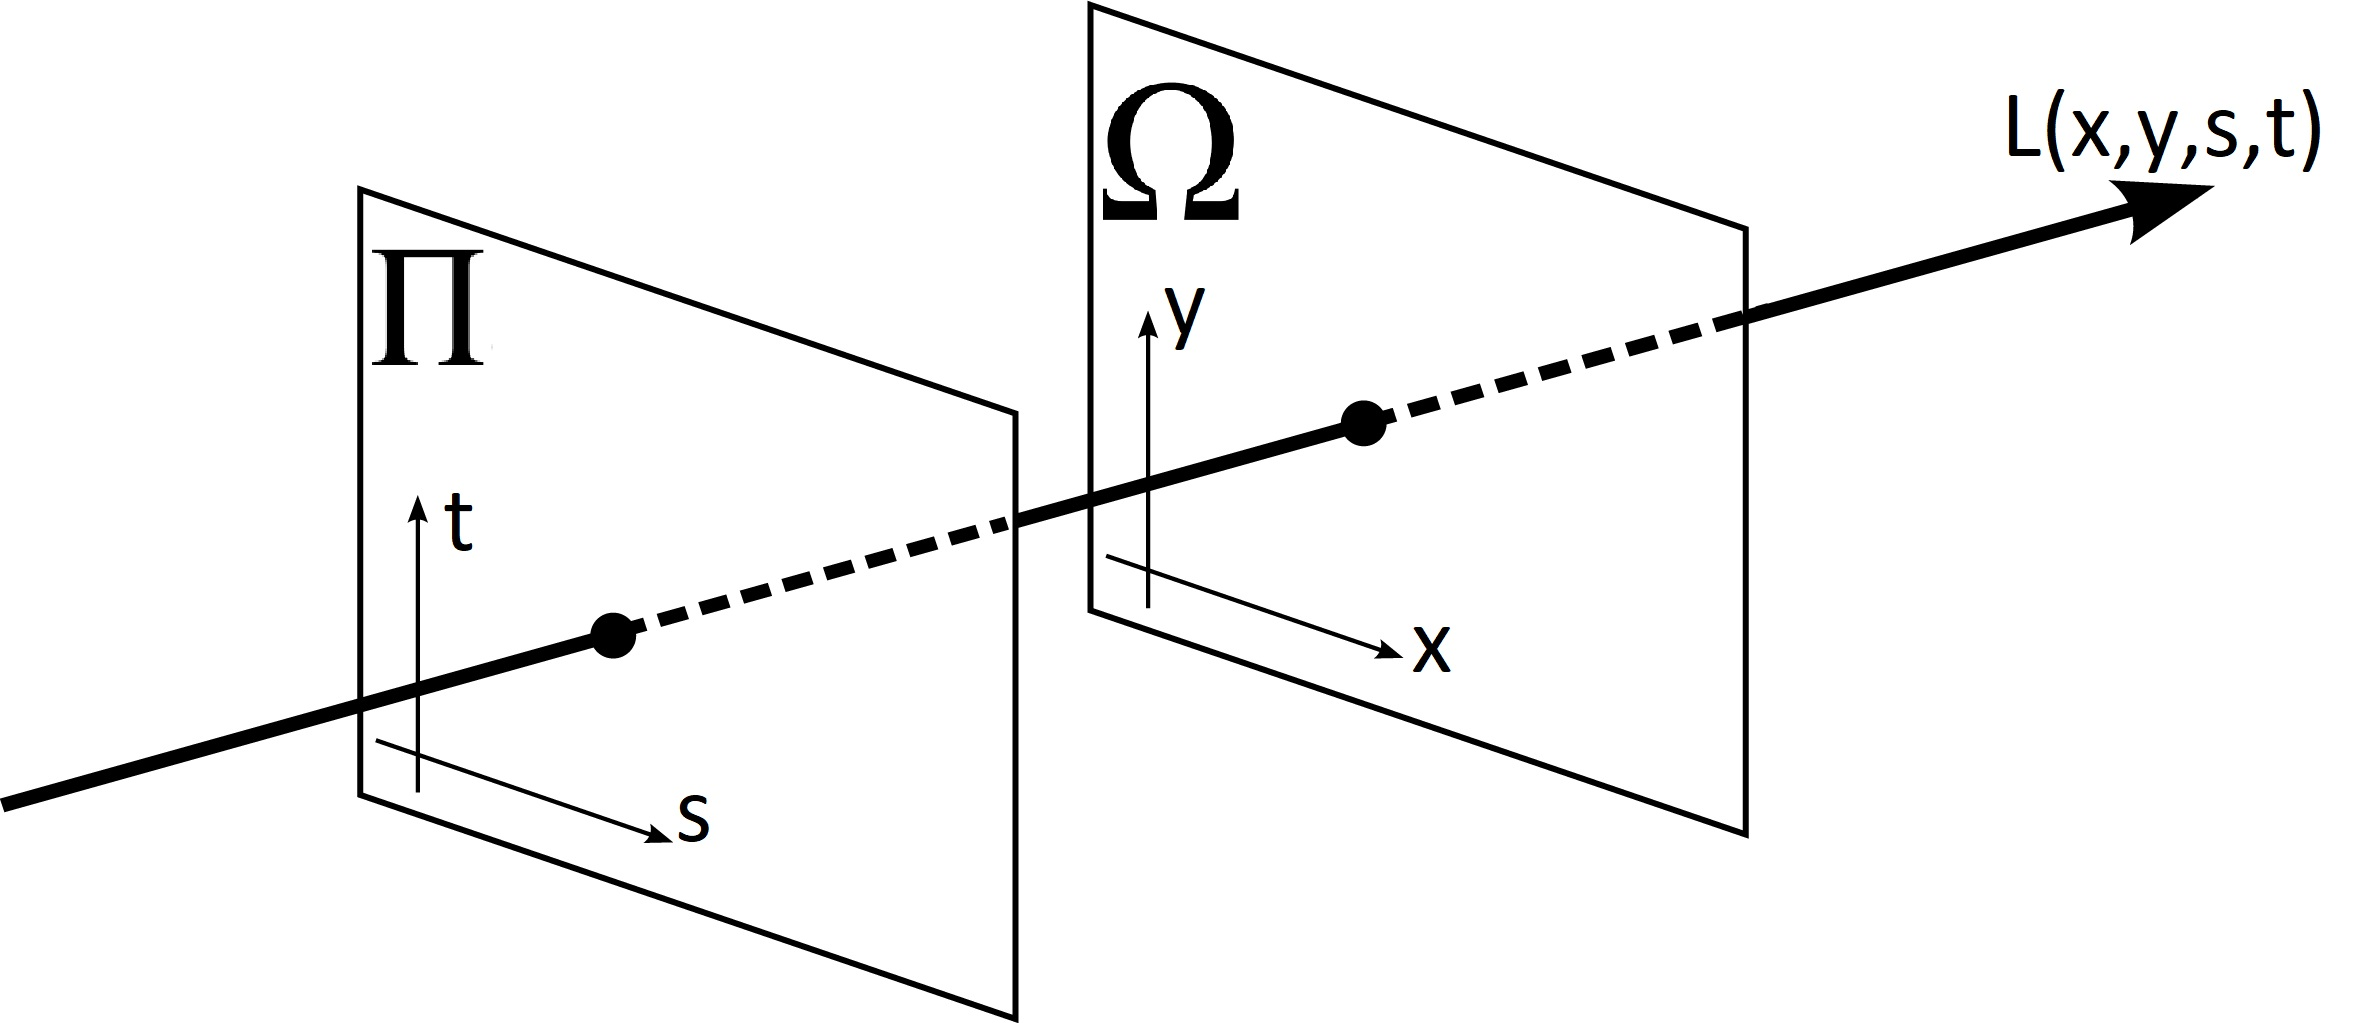
\includegraphics[width=0.7\linewidth]{images/twoplane_param}
	\caption[Two-plane parametrisation]{In a 4-dimensional two-plane parametrisation a light ray is characterized by the intersection with two parallel planes. we refer to the plane  $\Pi$ as the camera plane and the plane $\Omega$ as the image plane. From \cite{Xu:12}}
	\label{fig:twoplaneparam}
\end{figure}

\subsection{Epipolar Plane Images}
\label{sec:epi}
We measure the light field in order to obtain as much information about the scene we're looking at as possible. In order to obtain the threedimensional structure one needs to map the light field in a certain manner: We take a look at one 2-dimensional slice through the 4-dimensional space while keeping 2 coordinates constant: one horizontal coordinate  $x^{*}$  in the image plane and one vertical coordinate $t^{*}$ in the camera plane (or vice versa). The slice $\Sigma_{x^{*}, t^{*}}$ is a 2-dimensonal image called Epipolar Plane Image (EPI). In figure \ref{fig:epivisualization} the extraction of an EPI from camera array data is visualized. As seen in figure \ref{fig:simpleepi} it consists of lines with different slopes, each point on one line with the same slope belongs to the same point in the scene und different angles. From the slope $\Delta$ of the line at each point we obtain the distance from the camera plane with the equation
\begin{equation}\label{eq:distance}
\text{distance} = \frac{f\cdot b}{\Delta},
\end{equation}
where $f$ is the focal length of the camera and $b$ is the baseline between the camera positions. One may notices that this equation looks equal to distance estimation in stereo vision, where we replace the slope $\Delta$ by the disparity shift of a feature in 2 views. In fact, a stereo light field capture would result in an EPI with only 2 pixel rows, the slope of a line consisting of only two points is then defined as the disparity shift between the views.

\begin{figure}
	\centering
	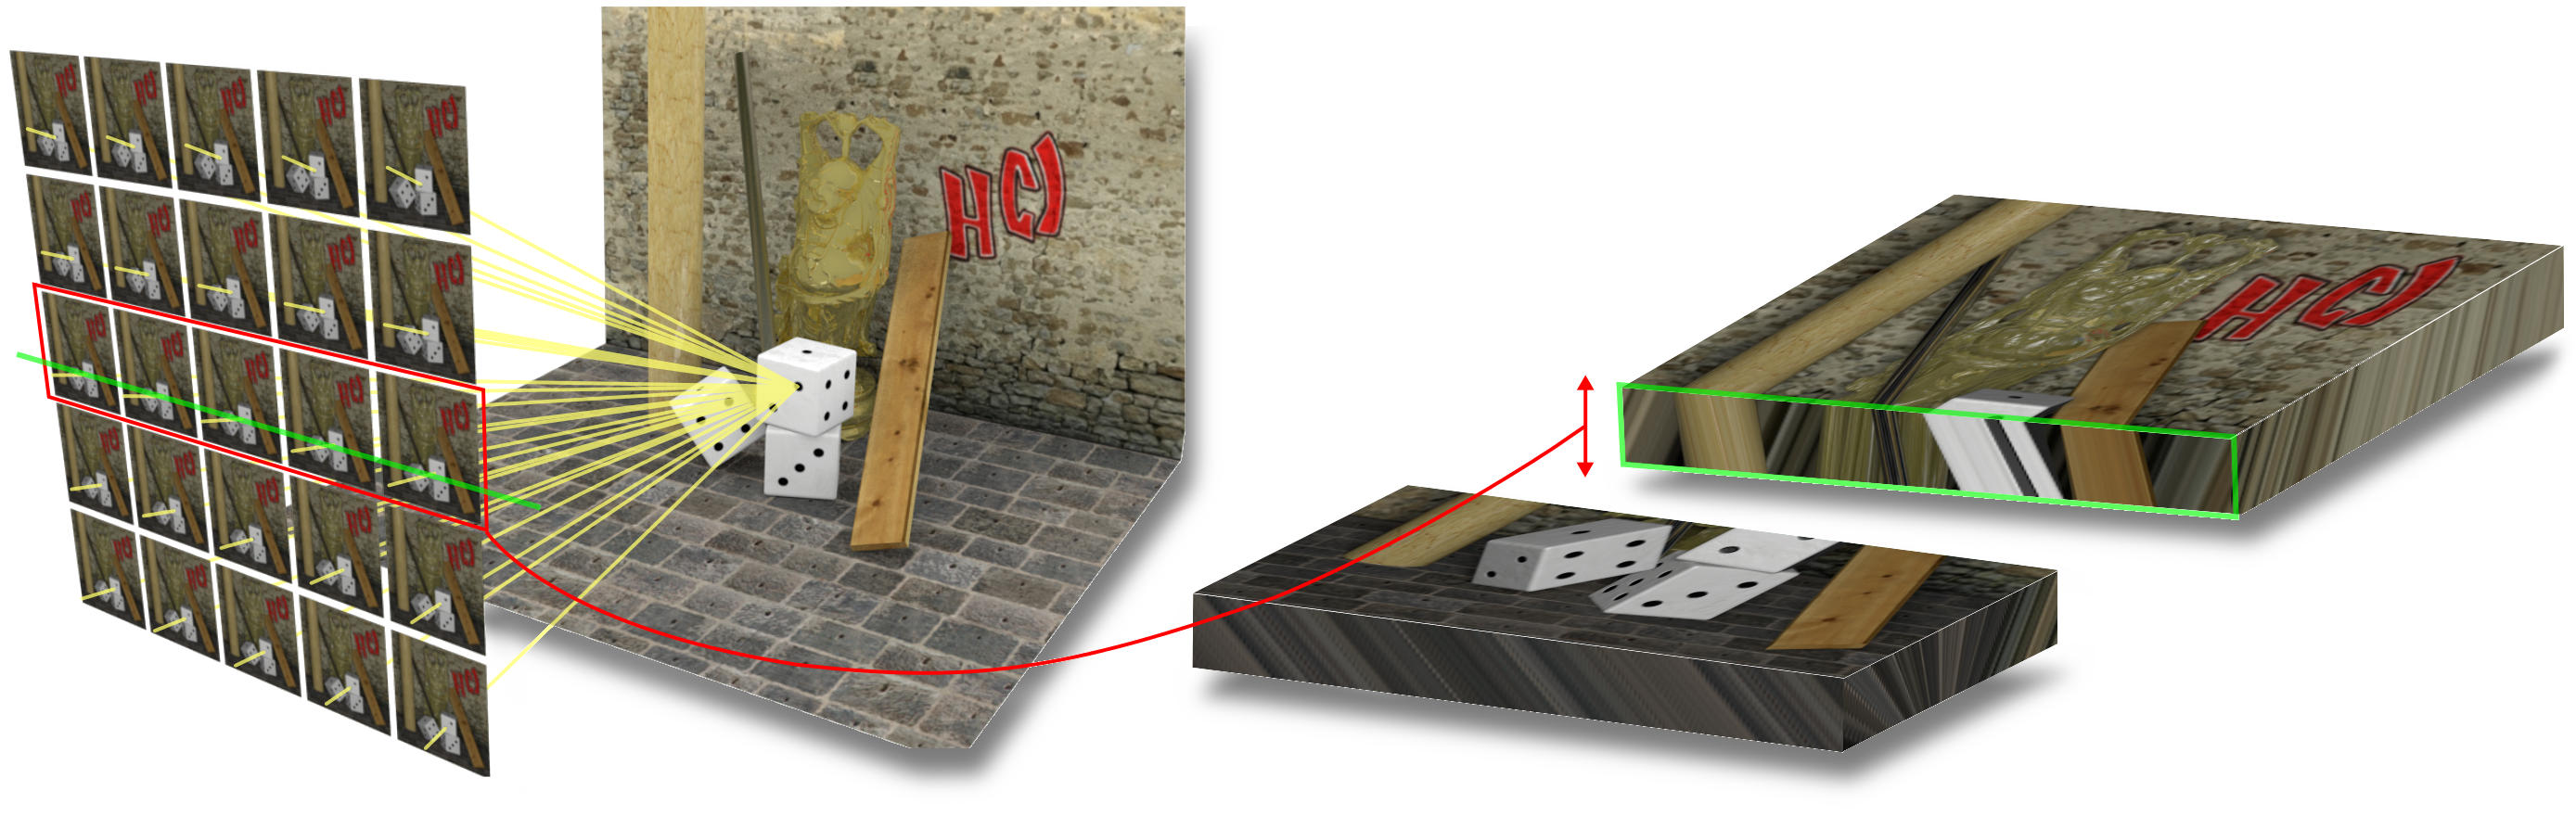
\includegraphics[width=1\linewidth]{images/epiVisualization}
	\caption[Visualization of an EPI extraction]{Visualization of an Epipolar Plane Image extractoin: A camera array takes images of the same scene from slightly different angles (left array). For a fixed image coordinate $y^*$ (green) and a fixed camera coordinate $t^*$ (red) the pixels are extracted and stacked up resulting in an EPI $\Sigma_{y^*, t^*}$ (green box on the right). From   \setcitestyle{numbers}\cite{iwr.uni-heidelberg.de} \setcitestyle{authoryear}}
	\label{fig:epivisualization}
\end{figure}

\begin{figure}
	\centering
	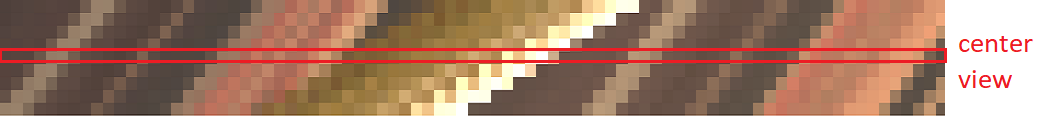
\includegraphics[width=1\linewidth]{images/simple_epi}
	\caption[Example Epipolar Plane image]{An Epipolar Plane Image (EPI) that consists of 9 rows (9 equidistant views or sample points in the camera plane). Points with the same color correspond to the same scene point. Since the viewpoints are slightly shifted, the scene point is also shifted in each view by the disparity $d$. Marked in red one can identify the center position of the camera viewpoints.}
	\label{fig:simpleepi}
\end{figure}

\section{Depth from Structure Tensor}
Measuring depth from light field data can be done using various approaches.
\cite{wu2017light} divide light field depth estimation approaches in three categories:
\begin{enumerate}
	\item Sub-Aperture Image Matching-based Methods
	\item EPI-based methods
	\item Learning-based methods
\end{enumerate}
In the following we focus on one specific EPI-based method on which is investigated as part of this work. However, the reader is encouraged to take a look at the cited paper \glqq Light Field Image Processing: An Overview \grqq by \cite{wu2017light} for a state-of-the-art overview of different light field approaches.\\
\cite{wanner2014orientation} makes use of the oriented structure of the EPI using image-processing techniques. This idea has first been introduced by \cite{bigun1987optimal} in 1987.\\

The 2-dimensional structure tensor $J$  on a function $g:\Omega \rightarrow \!R, \Omega \subset \!R^2 $ is defined as
\begin{equation}\label{eq:structuretensor}
J =\left(
\begin{matrix}
G*\frac{\partial g}{\partial x}\frac{\partial g}{\partial x} & G*\frac{\partial g}{\partial x}\frac{\partial g}{\partial s} \\
G*\frac{\partial g}{\partial s}\frac{\partial g}{\partial x} & G*\frac{\partial g}{\partial s}\frac{\partial g}{\partial s} 
\end{matrix}\right),
\end{equation}
 where $G$ is a gaussian window function. The derivation can be found in the appendix.
 The first eigenvector of this tensor $J$ indicates the preferred orientation in the local neighbourhood (defined by the window function). The second eigenvector is orthogonal to the first. 
 
   \cite{jahne2013digitale} proposes a coherence value as a measurement for the anisotropy of the local environment:
 \begin{equation}\label{eq:coherence}
 C = \frac{\sqrt{(J_{11} - J_{22})^2 + 4J_{12}^2}}{J_{11} + J_{22}}
 \end{equation}
 which obeys the value 1 in case of complete anisotropy, a value of 0 would indicate total isotropy.\\
 In case of an EPI, the structure tensor provides an estimate for the slope of an EPI line, as defined by \cite{bigun1987optimal}:
 \begin{equation}\label{eq:disparity}
 \Delta = \tan\left(\frac{1}{2} \arctan\left( \frac{J_{22}-J_{11}}{2J_{12}}\right)\right)
 \end{equation}
 we refer to $\Delta$ as the disparity $d$ in the following. Via equation \ref{eq:distance} one obtains the depth in meters.
 
 \subsection{Implementation}
 The following implementation steps have been proposed by \cite{wanner2014orientation}. The code uses \textit{crosshair} light field data, that can be obtained e.g. by a camera as depicted in figure \ref{fig:lumiplus}. The scope of the light field in the camera coordinates is significantly reduced, in the following the horizontal camera row and the vertical camera column are viewed seperately as 1-dimensional light-field cameras.\\
 \begin{figure}[]
 	\centering
 	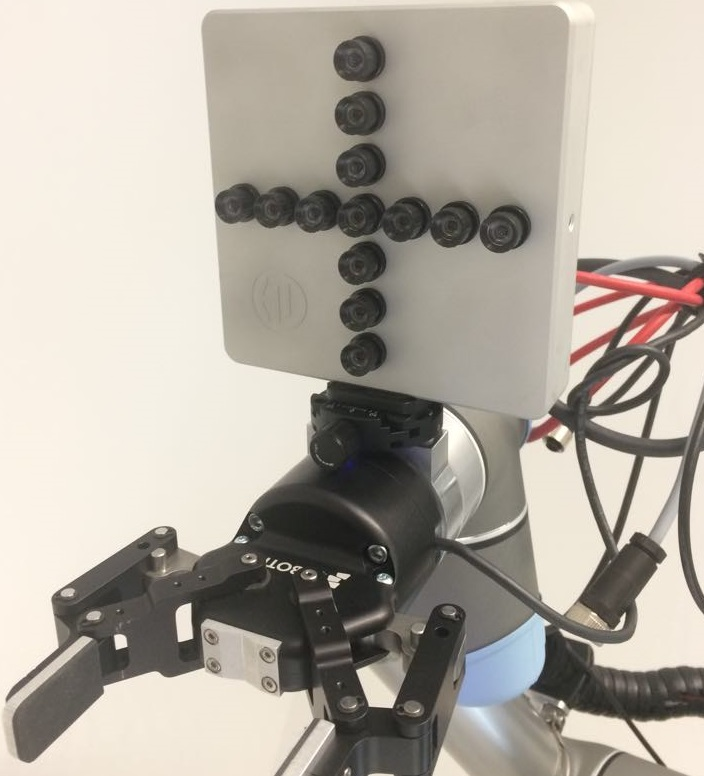
\includegraphics[width=0.7\linewidth]{images/Lumiplus}
 	\caption[LumiPlus Scanner from HDVisionSystems]{Instead of a complete camera array a crosshair camera reduces the number of cameras to one row and one column for faster processing. This Scanner from HDVisionSystems is mounted an a robot arm for industrial applications.}
 	\label{fig:lumiplus}
 \end{figure}
 
 From the input images one extracts the EPIs, which have the dimensions
 \begin{align*}
 \text{vertical view}&\rightarrowtail \text{Nr of rows in image coordinates }\times \text{Nr of cameras}\\
 \text{horizontal view}&\rightarrowtail \text{Nr of columns in image coordinates }\times \text{Nr of cameras}
 \end{align*}
 
 For each EPI we calculate the structure tensor independently. This is done by first presmoothing the EPI with a $3\times3$ gaussian kernel to obtain reasonable results when calculating the gradient in the next step. Note that before calculating the gradient, the EPI is converted to grayscale format.\\
 The gradient is calculated via the Scharr-filter, which has the form
 \begin{align}\label{key}
 \text{Scharr}_x &= \left(\begin{matrix}
 3&0&-3\\
 10&0&-10\\
 3&0&-3
 \end{matrix}\right)
\\
 \text{Scharr}_y &= \left(\begin{matrix}
 3&10&3\\
 0&0&0\\
 -3&-10&-3
 \end{matrix}\right).
 \end{align}
 \cite{wanner2014orientation} and \cite{diebold2016light} both tested out different gradient filters and came to the conclusion that the Scharr-filter performs best. With the gradients the structure tensor and the disparity is obtained via equation \ref{eq:structuretensor} and \ref{eq:disparity}.\\
 Further Wanner found out that the structure tensor results are most accurate when the disparity is close to zero. Therefore the EPI is artificially refocussed by simple linear shifting of the rows such that the slope of any line in the EPI would be increased by the same amount. The disparity shift can simply be subtracted from the disparity later. The refocussing of the EPI is illustrated in \ref{fig:refocusedcut}. For each EPI the structure tensor is calculated at each disparity shift, so that the necessary disparity range is fully covered.  \\
 \begin{figure}
 	\centering
 	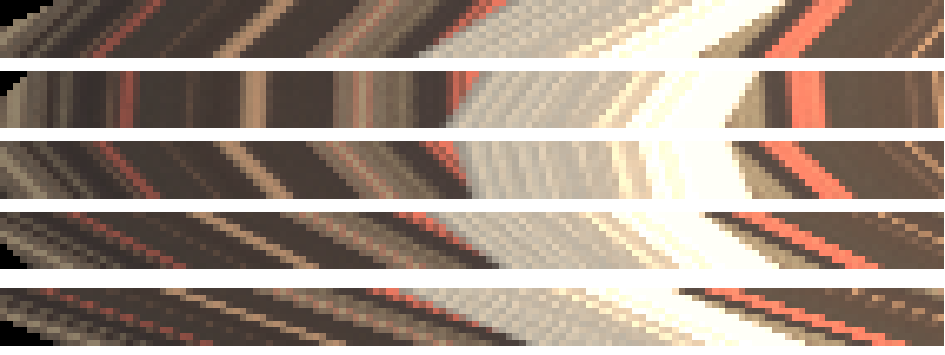
\includegraphics[width=0.7\linewidth]{images/refocused_cut}
 	\caption[Refocussed EPI]{The EPI is refocussed by integer disparity steps. If the slope at a scene point is zero (vertical line) the EPI is perfectly focussed on that point. An integration of all views would still result in a sharp image at the corresponding depth.}
 	\label{fig:refocusedcut}
 \end{figure}
 
 From all disparity shifts the value with the highest coherence measure (equation \ref{eq:coherence}) is selected. Hence one obtains two depth estimations for each image coordinate in the center view: one from the vertical EPI, one from the horizontal EPI. The merging of both direction follows
 \begin{equation}\label{key}
 d(x,y) = \begin{cases} d_\text{horizontal}(x,y) & C_\text{horizontal}(x,y)>C_\text{vertical}(x,y)\\
 						d_\text{vertical}(x,y) & C_\text{horizontal}(x,y)<C_\text{vertical}(x,y)\\
 		\end{cases}.
 \end{equation} 
 \subsection{The occlusion problem of the structure Tensor}
 \label{sec:occlusionproblem}
 Having a look at the results of the the benchmark test of \cite{honauer2016benchmark} one realizes that most Light field depth estimation algorithms suffer from large errors near depth discontinuities. Since the center view pixels close to the edge of a depth discontinuity are at least partly occluded, this behaviour is to be expected. The ST almost always produces a systematic error near discontinuities, leading to a \glqq magnification\grqq of the object closer to the camera in the depth map, see figure \ref{fig:cottondiscontinuities0070}. We refer to this as \glqq edge fattening \grqq. The reason for this error has its origin in the smoothing of the EPI as part of the algorithm.  At the occlusion, the edge between the fore- and background follows the same orientation as the foreground does. \\
  Furthermore the occlusion mostly comes with a a color change, resulting in a high gradient which dominates the local environment orientation: Edge fattening is the consequence. In figure \ref{fig:occlusion} one can recognize two effects leading to edge fattening: Firstly the EPI is smoothed with a $3\times 3$ gaussian kernel which already will enlarge the foreground structure (b). This becomes clear when we illustrate the norm of the gradients (c), since the strong (white) gradients all measure the forground (green) structure. A clear shift to the left is visible from (b) to (c). However, this bias error is small compared to the second error that is indicated in (d): The red dot lies clearly in the background structure. However, calculating the structure tensor components from the local environment (green square) one would obtain the foreground structure at the red dot, since the strong gradients in the square dominate. In (e) the total bias in labeling the two structures is illustrated. 
  \begin{figure}
  	\centering
  	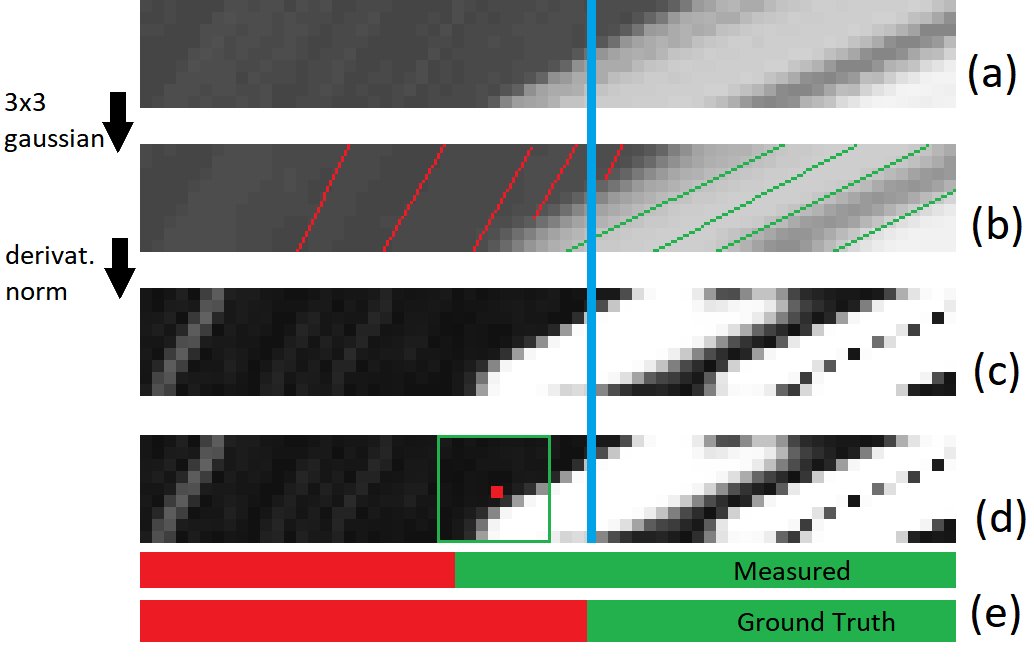
\includegraphics[width=0.7\linewidth]{images/occlusion_painted2}
  	\caption[Occlusion in an EPI]{(a) The structure of an occlusion border in a gray-value EPI. (b) Before calculating the gradient, the EPI is smoothed with a $3 \times 3$ gaussian kernel. One sees the smoothed EPI with colored lines indicating the Ground Truth orientation. (c) shows the norm of the gradient calculated via the Scharr-filter. White significates a high gradient, black significates low gradient. In (d) the local environment around the red dot $(x_r,y_r)$ as an example point is marked to show which gradient values go into the structure tensor components $J(x_r,y_r)$. (e) marks the orientation labeling measured and ground truth. The blue line marks the transition in the center view that corresponds with the ground thruth labeling. }
  	\label{fig:occlusion}
  \end{figure}
\begin{figure}
	\centering
	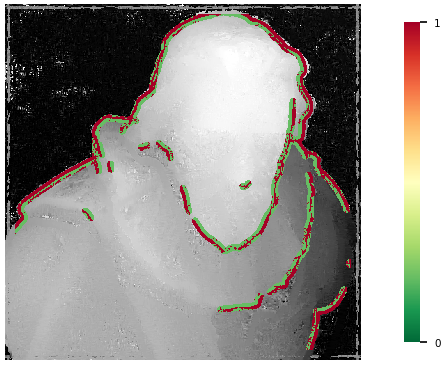
\includegraphics[width=0.7\linewidth]{images/cotton_discontinuities_0070}
	\caption[Discontinuity evaluation]{Evaluation of the deviation from Ground truth at the depth discontinuity for scene "cotton". The red border indicates that the depth map is errorneous at the outside of the edge.}
	\label{fig:cottondiscontinuities0070}
\end{figure}
  
 \section{Modifications on the structure tensor}
 In the following diffent methods will be explained which modify the Structure tensor algorithm proposed by \cite{wanner2014orientation}. In section \ref{Evaluation} implementations of those modifications will be evaluated and discussed.
 \subsection{Kernelsizes}
 The Structure tensor algorithm calculates the depth based on the preffered orientation of the EPI in a local neighbourhood. If one chooses a bigger neighbourhood, the resulting depth map is likely to be smoother, however the accuracy at edges in the scene will rapidly decrease.\\
 Even though one often wants to smoothen the depth map in a postprocessing step to improve the overall result and cancel out outlyiers, the structure tensor algorithm by Wanner is forced to smoothen the depth map beforehand.\\
 In the work of \cite{wanner2014orientation} the effect of the kernel size has been examined extensively and he calculated the best parameters for different scenes by grid search.\\
 Note that if the kernel is smaller then the height of the EPI, the outer cameras are neglected and do not enter in the calculation of the depth. To maintain the information of all cameras and vary the kernel size at the same time, \cite{diebold2016light} proposes asymmetrical kernelsizes to eventually reduce edge-fattening effects. However, assymetrical kernels still need to find a trade off between denoising and avoiding edge fattening and do not significantly increase the quality of the depth map result.\\
 Another approach is to choose a custom kernel form which only weights the local gradients that could possibly be part of the \glqq correct\grqq line in the EPI. Such a kernel is illustrated in figure (FIGURE), it has the form of as sandclock. in y-direction, it still follows a gaussian distribution.
 \subsection{Color-awareness with bilateral filtering}
 \label{sec:bilateral}
 In its original form the structure tensor pipeline weights the square of all gradients in a local environment by the distance to the reference point. Since all local gradients in the EPI that belong to the same color in the EPI are very likely to belong to the same orientation, in theory one only has to find all points with the same color which then lie on the same line in the EPI. The preferred orientation of the gradients at those points will then correspond to their slope with high confidence. However, most objects are not perfectly lambertian such that not all points on the correct line have to be of the exact same color. Only filtering the exact color will lead to noisy results. Though one could implement a filter weighting not only the distance in a gaussian manner but also the distance from the  EPI kernel origin in the color RGB space; such a filter is called \glqq bilateral filter \grqq (\cite{tomasi1998bilateral}). Pixels with completely different color will be excluded from the Neighbourhood when calculating the structure tensor. In equation \ref{eq:structuretensor} the window function $G$ is then defined as 
 \begin{equation}\label{key}
 G_P = \frac{1}{W_p}\sum_{q\in N} g_{\sigma_d}(||p-q||) g_{\sigma_c}(||I_{p, \text{EPI}}-I_{q, \text{EPI}}||),
 \end{equation}
 where
 \begin{itemize}
 	\item[$p$] is the position of the pixel,
 	\item[$q$] is the position of the pixel in a neighbourhood $N$,
 	\item[ $g_{\sigma_d}$] is a gaussian function weighting the distance between $p$ and $q$ using $\sigma_d$ as standard deviation,
 	\item[ $g_{\sigma_c}$] is a gaussian function weighting the color distance in RGB space between the  RGB values of the original EPI at $p$ and $q$ using $\sigma_c$ as standard deviation,
 	\item[$W_P$] is a normalization factor so that the sum over all the neighbourhood always is 1. 
 \end{itemize}
It is important to notice that the color distance is extracted from the EPI, though we are filtering the components of the second derivatives, see equation \ref{eq:structuretensor}. In fact, the EPI only serves as a \glqq guide\grqq for the filtering.
 \subsection{Thresholding the gradients}
 \label{sec:thresholdinggradients}
 In section \ref{sec:occlusionproblem} it is explained why the structure tensor struggles to serve with a  good estimation at depth transitions. It is referred to two errors, one coming from the first smoothing, the other one as a result from the second gaussian smoothing. To avoid the second error, one could in principle normalize all local gradients such that in figure \ref{fig:occlusion} (d) the foreground gradients in a local environment obey the same weight in the structure tensor calculation as the background gradients around the red dot.\\
 The gradient components of the EPI would be given by
 \begin{align}
 	\tilde{\vec \nabla}(x,y) = \frac{1}{\sqrt{\nabla_x(x,y)^2 + \nabla_y(x,y)^2}} \vec \nabla_x(x,y)
 \end{align}
 Nevertheless in some occasions one wants the stronger gradients to play a bigger role in the preferred orientation, since small gradients are more likely to be noisy. The only way to damp the gradients at occlusions while not strengthening the small noisy gradients in an EPI is to implement a trunctation threshold. The gradient is then given by
 \begin{align}
 \tilde{\vec \nabla}(x,y) &= \begin{cases}
\frac{\text{threshold}}{\text{norm}} \vec \nabla(x,y) \quad &\text{if}\quad \text{norm}> \text{threshold}\\
\tilde{\vec \nabla}(x,y) =  \vec \nabla(x,y)\qquad &\text{else}\\
 \end{cases} \\
\text{with} \quad \text{norm} &= \sqrt{\nabla_x(x,y)^2 + \nabla_y(x,y)^2}.\\
 \end{align}
 The threshold should be chosen the lowest possible in a manner that gradients higher than the threshold are barely affected by noise. In section \ref{sec:evaluation} different thresholds are tested, if not mentioned otherwise a threshold of 0.1 is used assuming that the underlying EPI is a gray-value image with range 0-1.\\
 
 \subsection{Occlusion-awareness using segmentation of the EPI}
 In the section a method is proposed that attempts to handle both occlusion errors mentioned in section \ref{sec:occlusionproblem}.\\
 Bilateral filtering (section \ref{sec:bilateral}) and thresholding the gradients (section \ref{sec:thresholdinggradients}) may improve the depth map estimation, however they come with trade-offs. See section \ref{sec:evaluation} for more details. An alternative way to maintain sharp transitions is to find those transitions in the EPI and calculating those seperately. By extracting them from the EPI, background and foreground structure are calculated without being biased by the transition itself. Therefor the EPI is segmented into occlusion transistions and areas, whereby the norm vector is thresholded to create a binary mask on the EPI. Possibly one could think of a better criterion that is segmenting occlusion/non-occlusion areas, however this approach is fastly implemented and is sufficient for our pipeline.
 
\begin{figure}
	\centering
	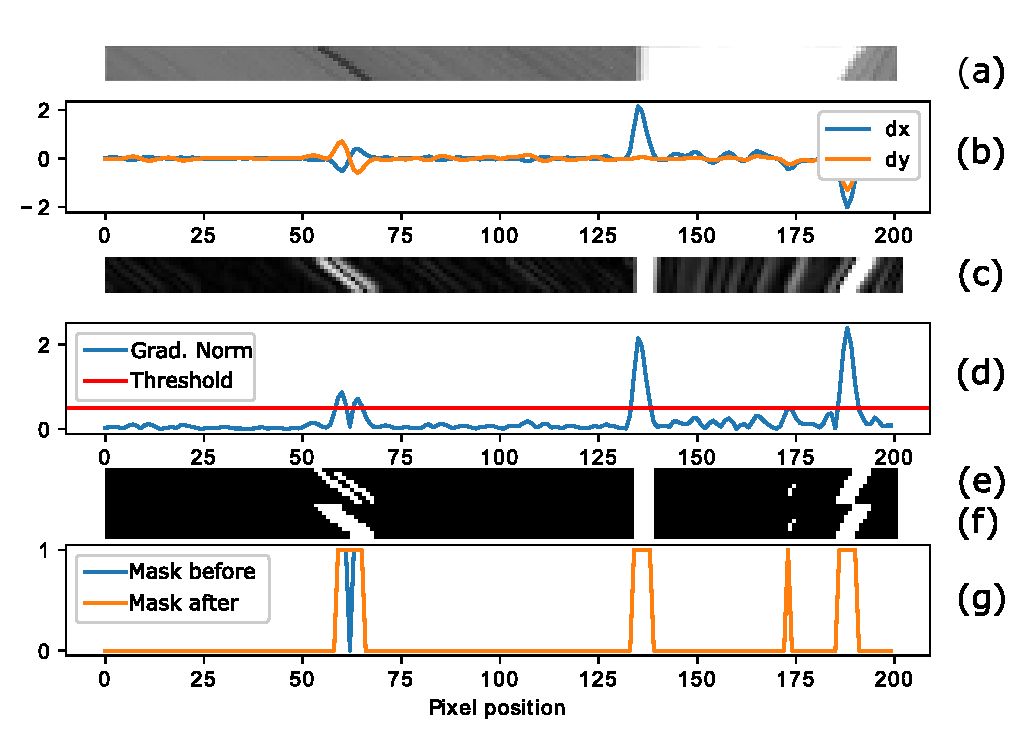
\includegraphics[width=1\linewidth]{images/derivatives_full}
	\caption[Segmentating an EPI]{(a) Input EPI to be segmented. (b) show the local derivatives along the center view line. (c) shows the vector norm of the derivative. (d) shows the center view norm with the threshold that is applyed to mask transitions. (e) shows the resulting mask. (f) shows the improved mask using morphological image processing. (g) shows the mask at the center view before and after using morph. image processing. }
	\label{fig:derivativesfull}

\end{figure}

\begin{figure}
	\centering
	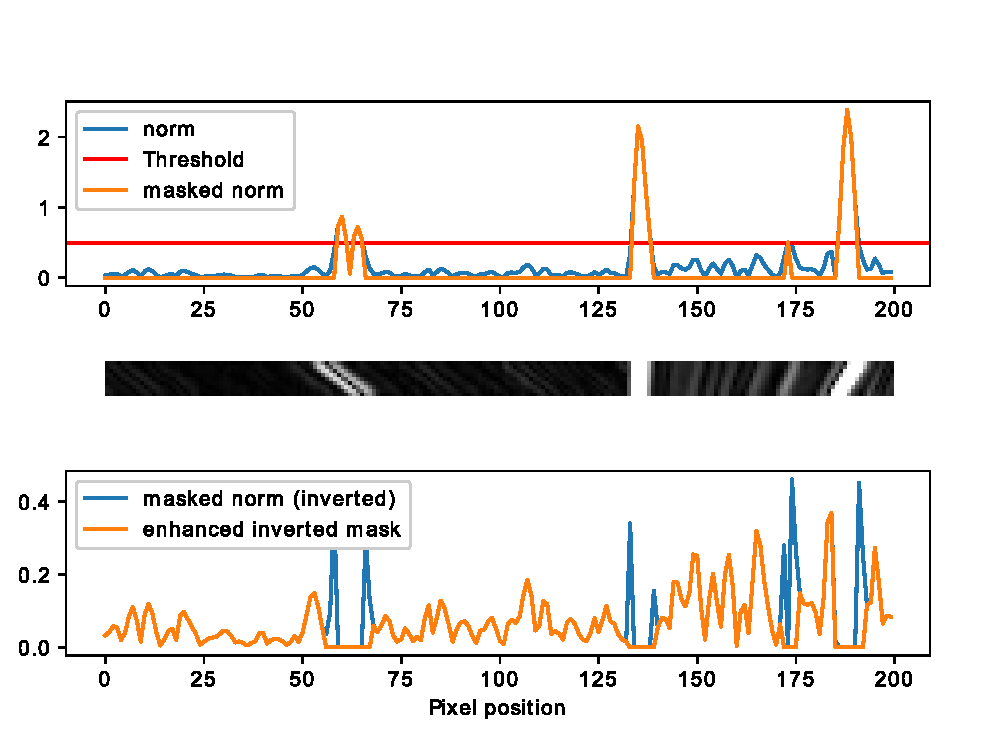
\includegraphics[width=1\linewidth]{images/segm_gaussian}
	\caption[Enhanced segmentation mask]{Enhanced segmentation mask}
	\label{fig:segmgaussian}
\end{figure}


 
 \subsection{An alternative to the coherence as the confidence measure}
\section{Depth from focus}
\label{sec:theo depth}
One advantage of using lightfields for depth measure is its ability to get a two-dimensional mapping of the scene with focus at any depth. Integrating the views of the light field camera array has the same effect as the integration of a focussed lense camera, as the lense is simply integrating slightly different viewpoints of the same scene point when focussed on the correct depth. \\
 Obtaining the refocussed integrated image is a synthetic process that only requires shifting the view coordinates artificially. Given a full four-dimensional light field $L(u, v, x, y)$ we can refocus the light field as described in\setcitestyle{numbers} \cite{ng2005light}\setcitestyle{authoryear}:
 \begin{equation}\label{eq:refocus}
L'(u, v, x, y) = L(u(1-d'), v(1-d'), x, y),
\end{equation}
where $d'$ describes the relative pixel shift. The disparity is directly related to the absolute depth of the focus (relate to PICTURE) if the relevant camera parameters are  known. Given the baseline $b$ in meters and the focal length $f$ in pixels, the depth $Z$ is given as \begin{equation}\label{key}
Z = \frac{f\cdot b}{d}.
\end{equation} 
We obtain
\begin{equation}\label{key}
\bar{L}(x,y) = \frac{1}{N_{u,v}}\int\int L'(u, v, x, y) du  dv =\frac{1}{N_{u,v}}\sum_{u}\sum_{v}  L'(u, v, x, y)
\end{equation}
Once we can focus at any range, one can adopt \textit{depth-from-focus}-techniques as described in \cite{watanabe1998rational} for depth measure. If the scene point at a given image coordinate $(x, y)$ in the center view is in focus, the contrast in the integrated image $\bar{L}(x,y)$ is high, thus a contrast measure at each pixel combined with stepwise refocussing yields a depth map. \\
For measuring the contrast, one has different options: The most straight forward approach is calculating the first derivative of the grey-value image. At high contrast structure the local intensity changes are expected to be high. Alternatively one could measure the second derivative laplacian that eventually results in higher robustness. The implementation and tests of those techniques for the benchmark dataset can be found in section \ref{label}.\\
Using a pinhole camera array allows us to go further and find a response value that shows higher consistency. Taking the absolute difference between the center view of the camera array and the refocussed image yields to promising results as shown in \cite{tao2017shape}. Under the assumption of lambertian surfaces the RGB- value of any scene point should be the same under all angles. Thus when refocussed on the correct depth, summing over all angles should result in a value that ideally is the same as in the center view alone. This is referred as \textit{photo consistency}; for more information read \cite{tao2017shape}.
The response value at a given depth is obtained from
\begin{equation}\label{key}
D'(x,y) = \frac{1}{|W_D|}\sum_{x',y' \in W_D} \left|\bar{L}(x',y')- P(x', y')\right|,
\end{equation}
where $P(x,  y)$ is the center view. For more robustness, it is averaged over a small window. We refer to this measuring technique as \textit{photo consistency} in the following. Note that calculating the absolute results in a 1-channel-image while the input images are RGB-images. \\ Tao et al. propose another measure that they refer to as \textit{angular correspondence}. It follows the same principle, but instead of integrating the refocussed lightfield followed by comparing it to the center view, they directly take the difference of each viewpoint to the center view and sum up those differences:
\begin{equation}\label{eq:responsecorr}
D'(x,y) = \frac{1}{N_{u,v}}\sum_{u}\sum_{v}  \left|L'(u, v, x, y) - P(x,y)\right|.
\end{equation}
We tested those methods against the common contrast measures mentioned above, the results are found in section results.

\section{Semi-Global Matching}
\subsection{Semi - Global Matching for Stereo Vision}
In contrast to Light field depth estimation techniques Stereo systems often suffer from mismatching pixels between the left and right images. Many attemps have been made to smoothen bad pixels, resulting in blurred edges or long calculation times. One promising attempt to imporove matching results was published in 2005 by Heiko Hirschmüller (\cite{hirschmuller2005accurate}) that was described as \glqq a very good trade off between runtime and accuracy \grqq $\,$ (\cite{hirschmuller2011semi}): we speak of Semi-Global Matching.\\
In general,  matching of two stereo images means shifting the disparity over the predefined disparity range and comparing both images (pixel- or blockwise) until we have a cost value at each image point for each discrete disparity. We assign to each pixel $\vec{p}$ the disparity value $D_{\vec p}$ which is related to the lowest cost $C(\vec{p}, D_{\vec p})$. This matching does not have to be unique, resulting in errorneous pixel disparities. 
To overcome this one wants to minimize a global cost function of the form 
\begin{equation}\label{eq:global_sgm}
E(D) = \sum_{\vec p} \left(C(\vec{p}, D_{\vec p}) + \sum_{q\in N_p} 
\begin{cases}
	P1 & \text{ if }|D_{\vec p} - D_{\vec q}| = 1\\
	P2 & \text{ if }|D_{\vec p} - D_{\vec q}| \geq 1\\
	0 & \text{ else }
	\end{cases}  
\right).
\end{equation}
The fist term sums all matching costs over the whole image, while the second term forces continuity by comparing the disparity of all neighbour pixels $N_q$ to the disparity $D_p$; if a  small discontinuity is detected ($D_{\vec p} - D_{\vec q} = 1$), a small penalty is added to the global cost function. Since a small discontinuity can be found essentially at any tilted plane, only a small error is added. A bigger disparity difference indices a clear discontinuity in the disparity map. Note that the penalty $P2$ can be divided by the gradient of the original image to allow a disparity discontinuity when we find edges in the image; at these points we expect the disparity to be discontinuous.\\ However, minimizing the global cost function involves computational cumbersome algorithms as it is a NP-complete Problem (\cite{hirschmuller2011semi}). Semi-Global Matching however chooses another approach by minimizing the global cost function along one-dimensional lines -- this can indeed be calculated in polynomial time.
The new smoothed cost function $S(\vec p , D_{\vec p})$ at pixel $\vec{p}$ is then given as the sum of all 1D minimum cost paths that are ending in $\vec{p}$.  The minimal cost $L'_r$ along the path $r$ is defined recursively as
\begin{equation}\label{eq:local_sgm}
L'_r(\vec{p}, D) = C(\vec{p}, D) + \text {min}
\begin{cases}
	L'_r(\vec{p_\text{before}}, D) \\
	L'_r(\vec{p_\text{before}}, D+1)+P1 \\
	L'_r(\vec{p_\text{before}}, D-1)+P1 \\
	\text{min}_i L'_r(\vec{p_\text{before}}, i)+P2 
\end{cases}
\end{equation} 
By always adding the minimum path cost of the previous pixel on the scanline we are looking at, we solve equation \ref{eq:global_sgm} in one dimension. It is to mention that the rolling sum can reach quite high numbers that are unpleasant to handle on the computer; a normalization is implemented by substracting min$_D L'_r(\vec{p_\text{before}}, D)$ from all pixel cost values $L'_r(\vec{p}, D)$. The position of the minimum cost function at pixel $\vec p$ is unaffected by that normalization.\\
 Summing along at least 8 path directions (crosshair + diagonals) results in disparity maps with reduced error pixel while maintaining clean edges. Neither a blur filter, a median filter or a bilateral filter would preserve those features.
\subsection{Semi - Global Matching for Light fields}
Even though Hirschmüller describes Semi - Global Matching (SGM) as a complete algorithm to obtain a disparity map from a stereo image input, we further refer to SGM as the true novelty of his work: the implementation of an approximation to the global solution of the cost function (equation \ref{eq:global_sgm}). Indepent from the method one uses to calculate a disparity map,  one needs a cost function defined in disparity space for each pixel to make use of SGM. 
Similar to the Stereo Matching depth estimation, the structure tensor depth estimation pipeline for Lightfield data sets produces a disparity map and a coherence value at each disparity shift. This implies, that the SGM algorithm can be adapted to improve the results of the structure tensor pipeline. However, there are some significant differences between those two methods:
\begin{enumerate}
	\item The structure tensor algorithm is tuned to a much smaller disparity range. While in \cite{hirschmuller2005accurate} Hirschmüller scans a disparity range of 32 pixels , The benchmark data sets for light fields mostly include close-up views of objects, with a disparity range between 2 and 10 pixels. In figure \ref{fig:table-skizze} one can see the different values that are allocated in memory for each pixel of the image.
	\item The subpixel accuracy using the structure tensor is a lot higher than the stereo matching subpixel accuracy. A simple adaption of the algorithm to the structure tensor pipeline would require to give up the best feature that is provided by the ST, its subpixel accuracy.
\end{enumerate}
\begin{figure}[h]
	\centering
	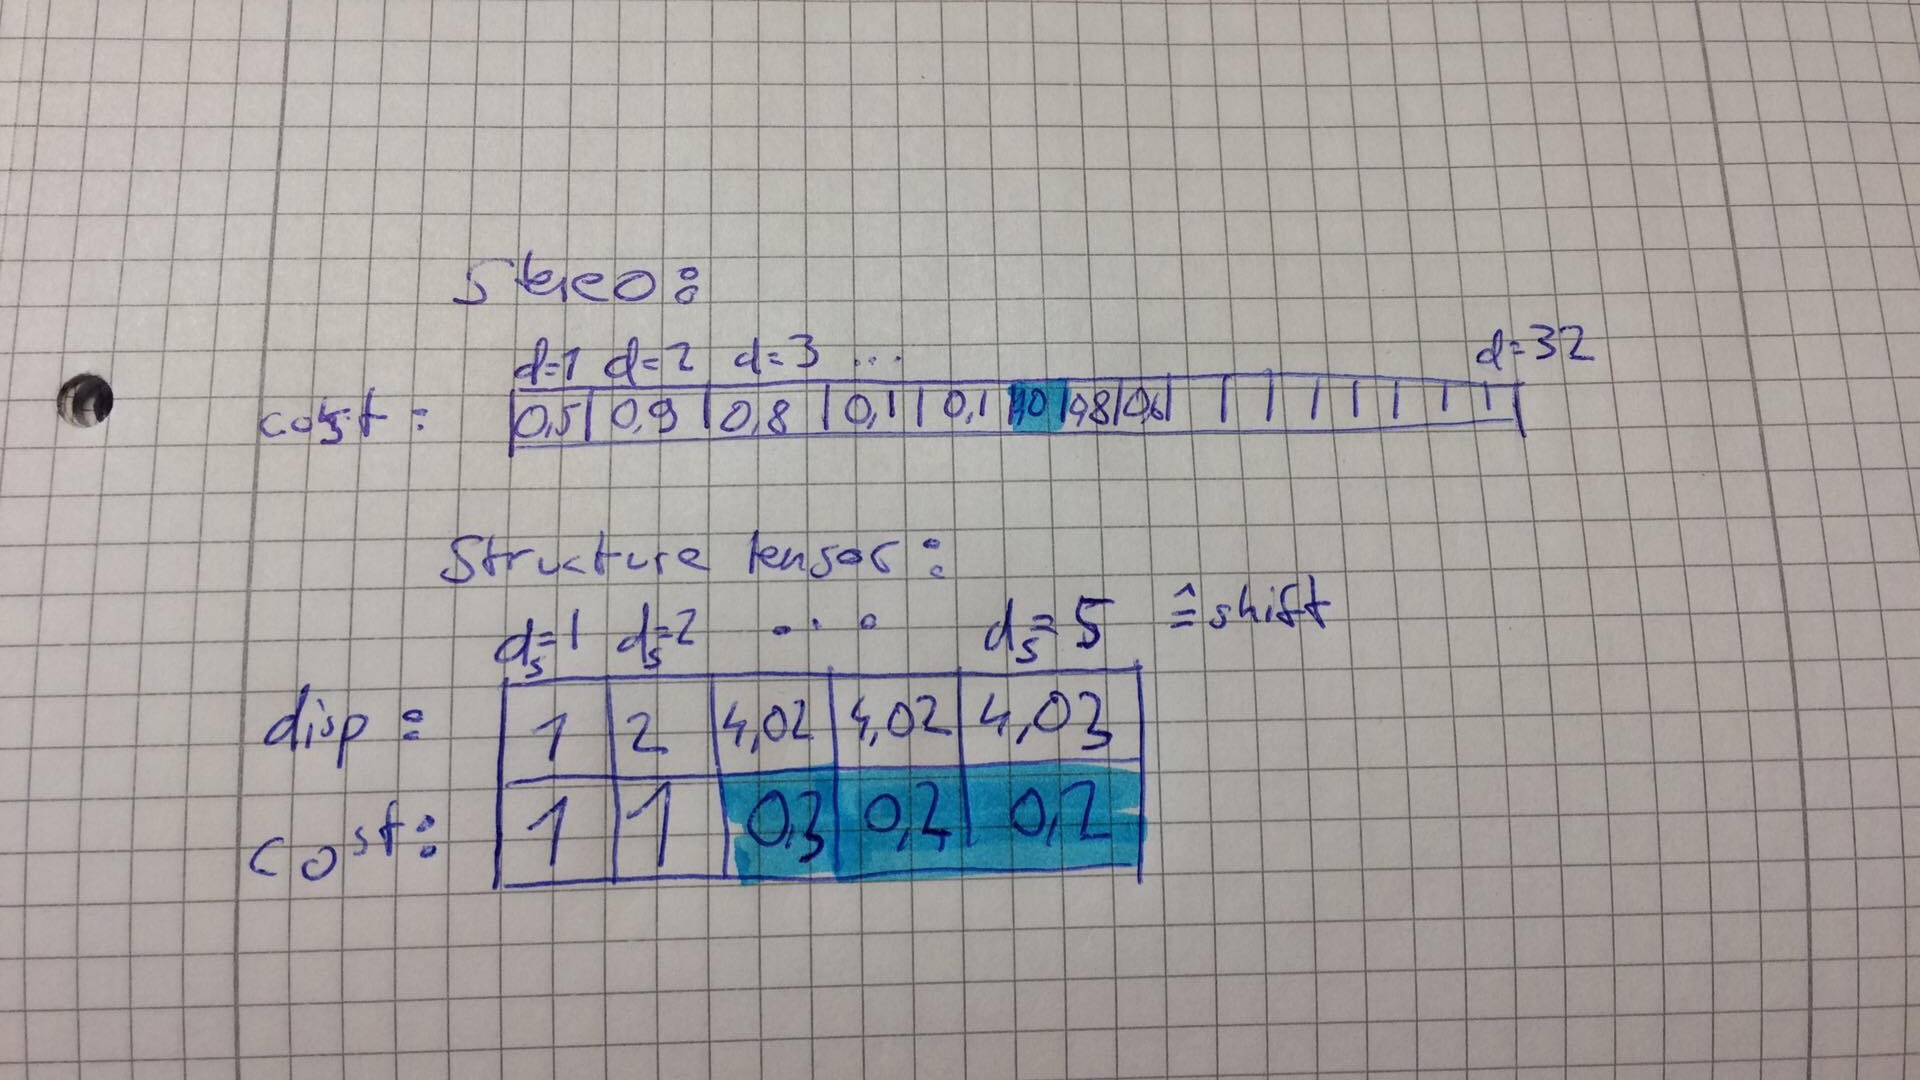
\includegraphics[width=0.7\linewidth]{images/table-skizze}
	\caption[Example values: One point $\vec p$ contains different values]{One point $\vec p$ contains different values (values here: example values): For Stereo matching, the resolution is given by the discrete disparity steps. Each disparity value has a cost value assigned to it. Using the ST, we have a different subpixel accuracy for every disparity shift, while the subpixel accuracy can differ from the shift by up to 1.2 }
	\label{fig:table-skizze}
\end{figure}

To handle those problems, we do not throw away the subpixel accuracy: instead we use the float-value disparities to decide whether we penalize a disparity discontinuity or not. As one can see in figure \ref{fig:table-skizze}, we have to process an additional information, since the exact disparity value is not implicitely given by the index of the allocated cost value (in contrast to the original algorithm). Switching to a continuous space as depicted in figure \ref{fig:discretecont} requires a new definition of the error propagation defined in equation \ref{eq:global_sgm}.
\begin{figure}
	\centering
	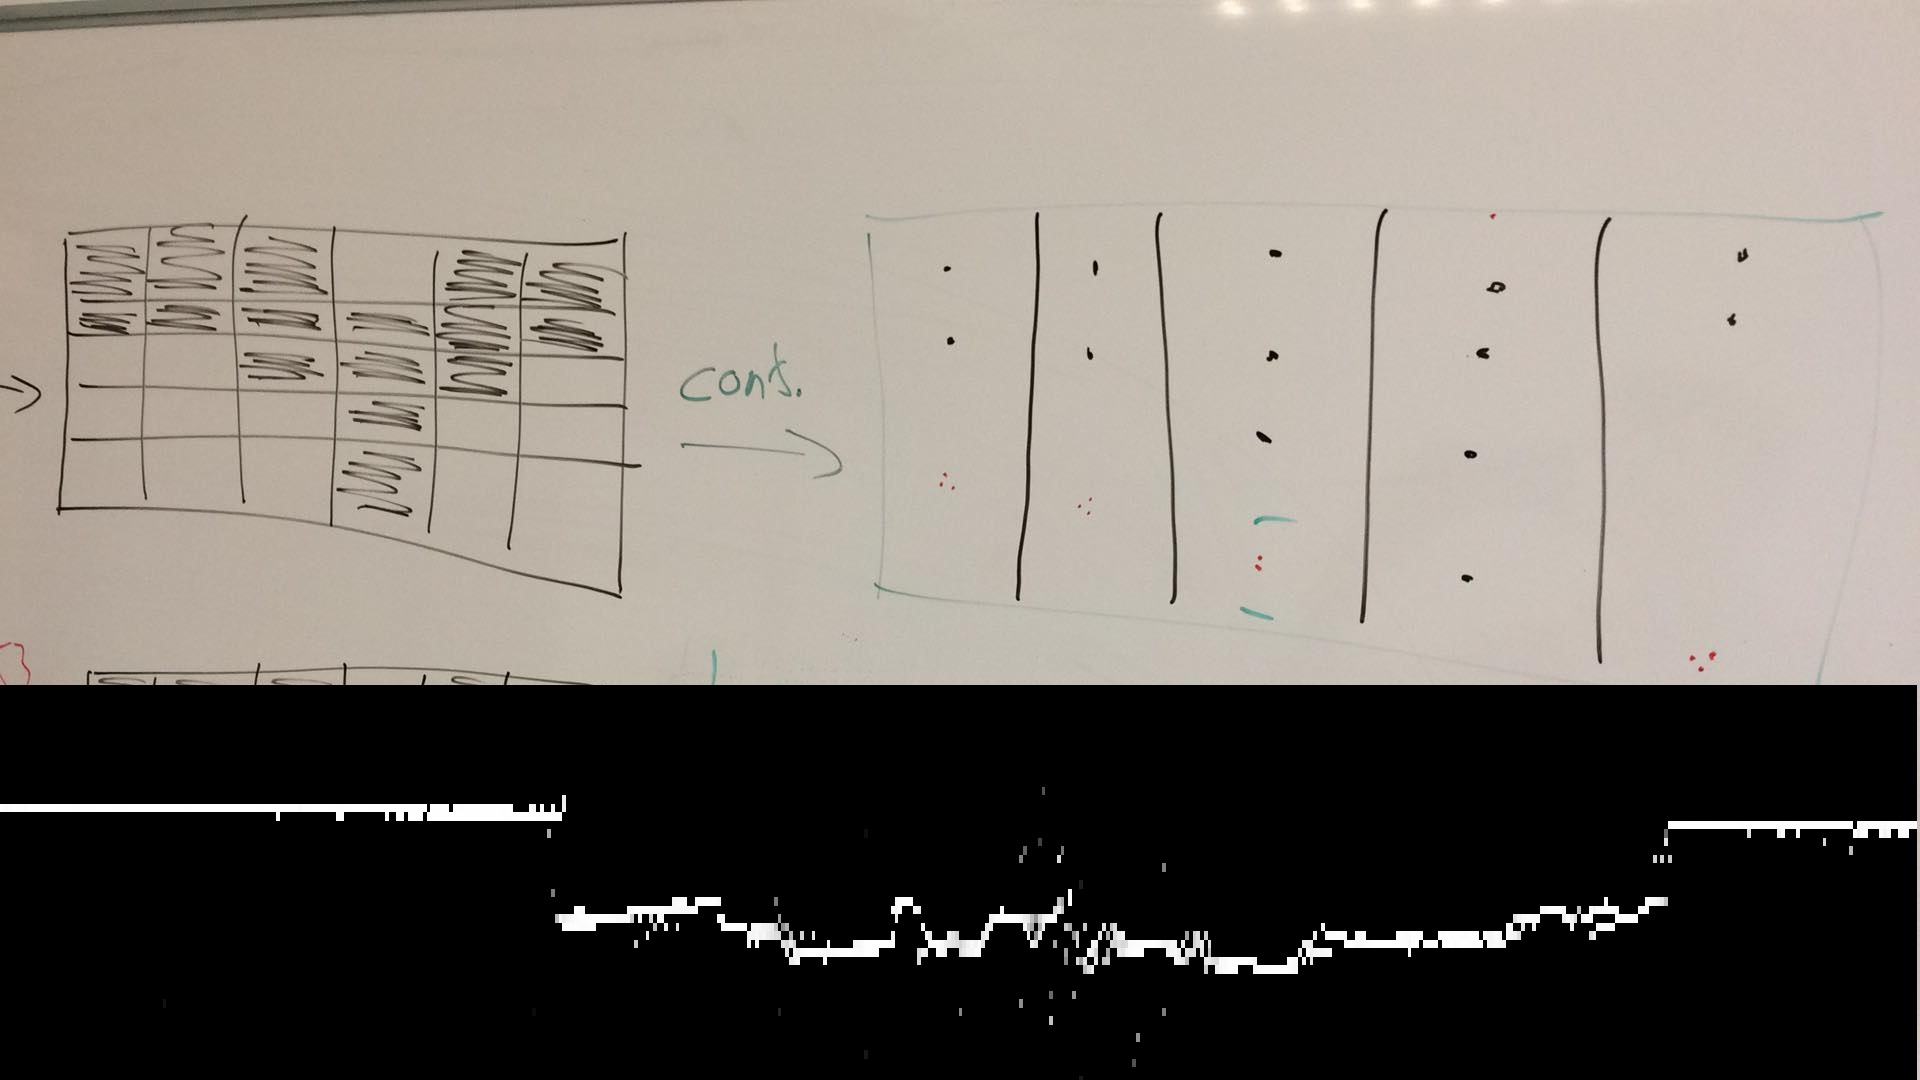
\includegraphics[width=0.7\linewidth]{images/discrete_cont}
	\caption[Discrete scanline to continuous scanline]{In this figure one can see the skizze of one arbitrary scanline of the structure tensor method. Under the Assumption that the ST algorithm recognizes the structure of the EPI perfectly, we either have two or three disparity shifts that have a high coherence (colored white) (a) and result in approximately the same final disparity. This can be seen if we plot the exact disparity values in a continuous space(b). In (c) real data scanline cost is plotted with a resolution of ca. 100 pixels.}
	\label{fig:discretecont}
\end{figure}


 In the following we refer to $s$ as the disparity shift in the ST algorithm. Note that we replaced $D$ by $d$ to clarify that the disparity is no longer discrete:

\begin{equation}\label{eq:global_sgm_cont}
E(d) = \sum_{\vec p} \left(C(\vec{p}, d_{\vec p}) + \sum_{q\in N_p} 
\begin{cases}
P1\cdot |d_{\vec p} - d_{\vec q}|  & \text{ if }|d_{\vec p} - d_{\vec q}| \leq 1\\
P2 & \text{ if }|d_{\vec p} - d_{\vec q}| > 1\\
\end{cases}  
\right).
\end{equation}
The recursive 1-d form to solve the global constraint on a scanline then changes to:

\begin{equation}\label{key}
L'_r(\vec{p}, s) = C(\vec{p}, s) + \text{min}_i
\begin{cases}
L'_r(\vec{p}_\text{before}, s_i)+P1 \cdot |d_{\vec p, s} - d_{\vec{p}_\text{before}, s_i}|  & \text{ if }|d_{\vec p, s} - d_{\vec{p}_\text{before}, s_i}| \leq 1 \\
L'_r(\vec{p}_\text{before}, s_i)+P2 & \text{ if }|d_{\vec p, s} - d_{\vec{p}_\text{before}, s_i}| > 1
\end{cases}
\end{equation} 
The biggest difference lies in the fact that the small factor that is smoothing the image linearely increases with the distance. This change is necessary under the assumption that the disparity space is continuous. In other words we cluster disparity differences between two neighbouring points as either part of one surface ($|d_{\vec p, s} - d_{\vec{p}_\text{before}, s_i}| \leq 1$) that gets smoothed by the linearly increasing penalty, or assume a real disparity discontinuity that is penalized regardless of the size of the jump - the second error remains constant as it is in Stereo matching. Note that in our implementation, $P2$ is modified by 
\begin{equation}\label{key}
P2' =  \frac{P2}{\sqrt{(Im_b^2 +Im_r^2 + Im_g^2)}},
\end{equation}
with $Im$ being the center view of the lightfield and $Im_{b,g,r}$ being the 3 color channels. If the color intensity changes, the penalty for a disparity discontinuity is lowered.

\subsection{Occlusion awareness in SGM for light Fields}

If we take a close look at figure \ref{fig:discretecont}, one can see that at least at some discontinuities the ST pipeline manages to calculate the depth of the background structure near boundaries with good coherence, but the foreground structure is overlapping and quantitatively measured with higher coherence. Once we know that at least at some edges an improvement can be made by adapting the evaluation function in a sense that the highest coherence does not necessarily measure the right depth, we realize that SGM is doing the job already. The simple heuristic approach is to change the global minimization function \ref{eq:global_sgm_cont} such that a positive disparity jump is less punished than a negative one. In fact, the function changes to
\begin{equation}\label{eq:global_sgm_cont_occlusion}
E(d) = \sum_{\vec p} \left(C(\vec{p}, d_{\vec p}) + \sum_{q\in N_p} 
\begin{cases}
P1\cdot |d_{\vec p} - d_{\vec q}|  & \text{ if }|d_{\vec p} - d_{\vec q}| \leq 1\\
P2 & \text{ if }d_{\vec p} - d_{\vec q} > 1\\
P3 & \text{ if }d_{\vec p} - d_{\vec q} < -1\\
\end{cases}  
\right).
\end{equation}
\subsection{SGM as postprocessing smoothing}



\chapter{Evaluation}
\label{Evaluation}
\section{Depth from focus}
\label{sec: depth from focus}
The depth measure using epipolar plane analysis requires iterative calculation of the structure tensor for each EPI at each disparity. A way to overcome this is to generate a preestimate of the depth before actually calculating the correct depth. This could also help to prevent possible errors due to periodic scene characteristics which can lead to mismatch errors when calculating the structure tensor. Therefore the depth pre-estimate should fulfil the following criteria:
\begin{enumerate}
	\item It should be \textit{consistent}, meaning that the number of pixels with low confidence should be the lowest possible.
	\item It should result in a \textit{fast} measure, ideally faster then it would take to do the full iterative structure tensor algorithm.
	\item It does not have to be subpixel accurate, since it only serves as a pre-estimate. 
\end{enumerate}

The methods that are tested are described in section \ref{sec:theo depth}. We test four different ways to obtain a depth map using depth from focus:
\begin{description}
	\item[Photo consistency] This measure takes advantage of the fact that the difference between the refocussed two-dimensional image and the center view is close to zero when refocussed to  the correct depth. Response value:
	\begin{equation}\label{key}
	D'(x,y) = \frac{1}{|W_D|}\sum_{x',y' \in W_D} \left|\bar{L}(x',y')- P(x', y')\right|,
	\end{equation}
	\item[Angular correspondence] In contrast to the \textit{Photo consistency} - measure, it first calculates the absolute difference between each camera array view and the center view followed by the summation of those deviations. The response value is given as in equation \eqref{eq:responsecorr}
	\begin{equation}\label{key}
	D'(x,y) = \frac{1}{N_{u,v}}\sum_{u}\sum_{v}  \left|L'(u, v, x, y) - P(x,y)\right|
	\end{equation}
	
	\item[First derivative] The first derivative is calculated for contrast measure by applying the sobel filter onto the refocussed image $I$:
	\begin{equation}\label{key}
	 G_x=
	 \left[ {\begin{array}{ccc}
	 	-1 & 0 & 1 \\
	 	-2 & 0 & 2 \\
	 	-1 & 0 & 1 \\
	 	\end{array} } \right] \cdot I \quad G_y=
	 \left[ {\begin{array}{ccc}
	 	-1 &-2 &-1 \\
	 	0 & 0 & 0 \\
	 	1 & 0 & 1 \\
	 	\end{array} } \right] \cdot I
	\end{equation} 
	The directional gradients are simply added up to the response value
	\begin{equation}\label{key}
	D'(x,y) = |G_x(x,y)| + |G_y(x,y)|
	\end{equation}
	\item[Laplace] Here we calculate the second derivative laplacian by appling the sobel operator twice:\begin{equation}\label{key}
	D'(x,y) = \text{Laplace}(I)(x,y) = \frac{\partial^2 I}{\partial x^2}(x,y) + \frac{\partial^2 I}{\partial y^2}(x,y)
	\end{equation}
	
	In the following we are going to compare the method qualitatively and quantitatively. In figure \ref{fig:originalmarked} one can see the pixel response value refocussed at different disparities for all the methods at example points in the testscene \glqq complextestscene\grqq. We chose points close to edges as well as points on clear surface with less structure on it. One can see that the pixel response of the Angular correspondence and the Photoconsistency method for those points show a more consistent behaviour, meaning that only one clear maximum can be seen. The derivative method as well as the Laplace method both seem to have trouble especially on pixel coordinates close to edges. This can be seen most clearly at the edge of the melon, where The first derivative shows 2 Maxima, while the Angular correspondence and Photo consistency measure find a clean maximum indicating at which depth the point can be found. However, on surfaces with less structure as for example on the potato, the Photo consistency measure struggles to find a clear maximum -- still it has one at the right position. 
	\begin{figure}
		\centering
		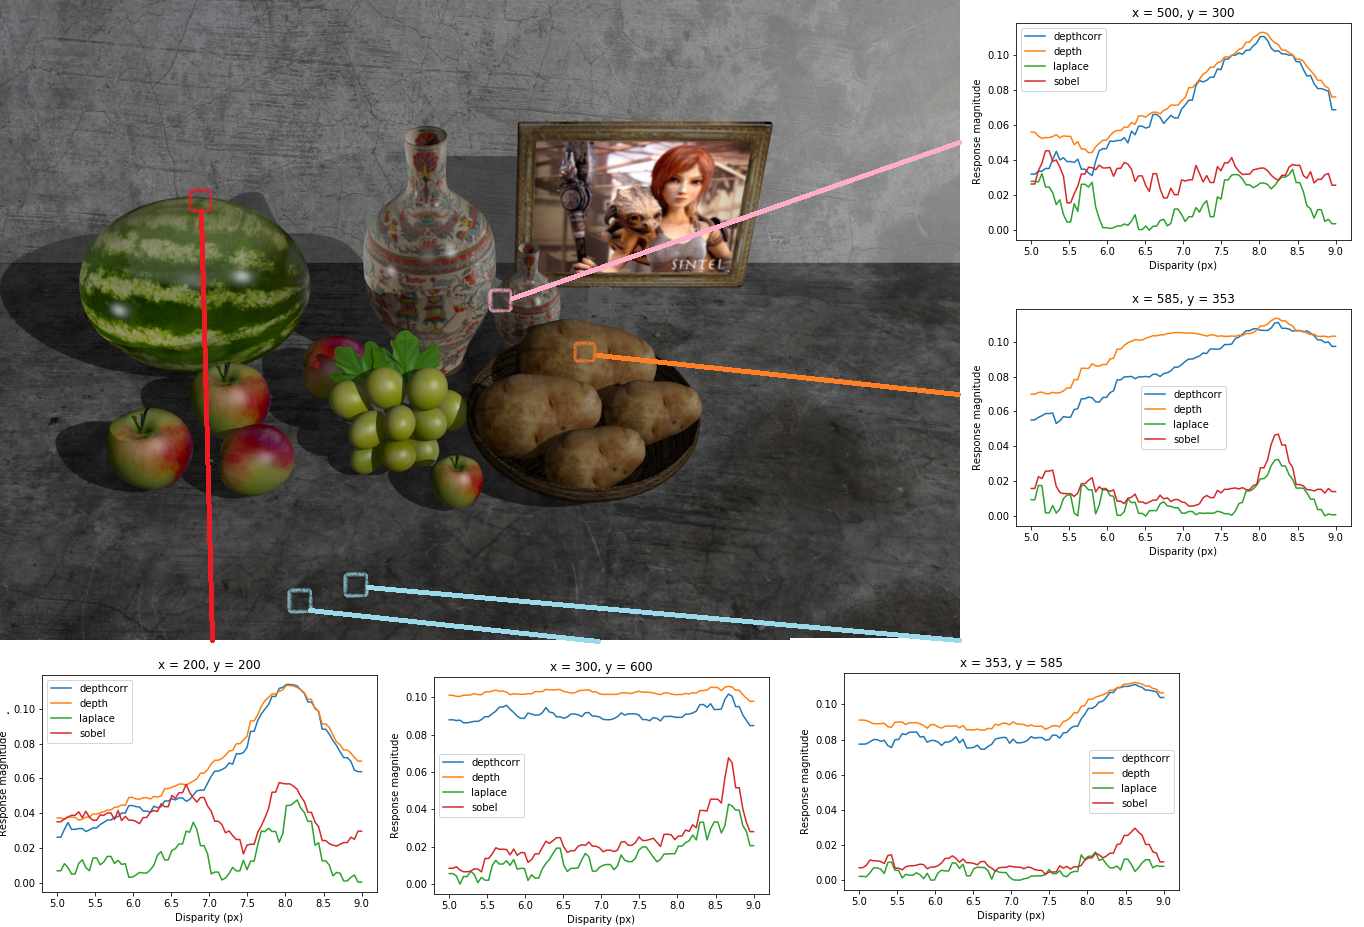
\includegraphics[width=1\linewidth]{images/original_marked}
		\caption[Pixel response for depth from focus techniques]{At different pixel positions we take a look on how the Pixel response value behaves for the four different depth-from-focus techniques: Photo consistency (orange), Angular correspondence ( blue), First derivative (red) and The Laplace method (green) A high value means high confidence (low cost).}
		\label{fig:originalmarked}
	\end{figure}
	Having a look at the actual disparity maps produced by the different techniques we can already
	capture that the angular correspondence and photo consistency method produce the more consistent, smooth disparity maps. A quantitative evaluation confirms this impression: We measure the mean relative error (MRE), which is defined as the mean squared error over all pixels $\vec{p}$ divided by the maximum disparity range (the maximum error possible).
	\begin{equation}\label{key}
	MRE = \sum_{\vec p } (d_{\text{ground truth}} - d_{\vec p} )^2/(\text{max. disp - min. disp})
	\end{equation}
	
	
	
	
	\subsection{Using depth-from-refocus as a preestimate for the ST}
	The long-term aim of this work is to make the structure tensor pipeline more robust. We achieve this by using the depth-from-refocus method as a pre
\end{description}

  \part{Appendix}
  \begin{appendix}
  	\section{Derivation of the structure tensor}
  	The derivation is taken from \cite{jahne2013digitale}. Taking a function $g:\Omega\rightarrow \!R, \Omega \subset \!R^D$, the pereferred local direction $\vec{n} \subset \!R^D$ must satisfy the following equation:
  	\begin{equation}\label{key}
  	( g^T\vec{n})^2 = |\nabla g |^2 \cos^2(\sphericalangle (g, \vec{n}))
  	\end{equation}
  	If $\nabla g$ is parallel or antiparallel to $\vec{n}$, the expression on the right side reaches a maximum. Therefor one needs to maximise the left hand expression in a local environment:
  	\begin{equation}\label{key}
  	\vec n_\text{preferred} = \argmax_n\left(\int w(\vec x - \vec x')\left(\nabla g(\vec{x'})^T \vec{n}\right)^2d^Dx' \right),
  	\end{equation}
  	$w$ is a window function defining the size of the local environment. Multipling with $\vec{n}$
  	we obtain:
  	\begin{align}\label{key}
  	&\vec n_\text{preferred} = \argmax_n\left(\vec n  J \vec n \right)\\
  	& J = \int w(\vec x - \vec x')\left(\nabla g(\vec{x'}) \nabla g(\vec{x'})^T\right)d^Dx'
  	\end{align}
  	This results in a $D\times D $ tensor of the form
  	\begin{equation}\label{key}
  	J_{pq} = \int_{-\infty}^{\infty} w(\vec x - \vec x')\left(\frac{g(\partial\vec{x'})}{\partial x'_p} \frac{g(\partial\vec{x'})}{\partial x'_q}\right)d^Dx'.
  	\end{equation}
  	In two dimensions we can write
	\begin{equation}\label{key}
	J =\left(
	\begin{matrix}
	w*\frac{\partial g}{\partial x}\frac{\partial g}{\partial x} & w*\frac{\partial g}{\partial x}\frac{\partial g}{\partial s} \\
	w*\frac{\partial g}{\partial s}\frac{\partial g}{\partial x} & w*\frac{\partial g}{\partial s}\frac{\partial g}{\partial s} 
	\end{matrix}\right),
	\end{equation}  
	where \glqq $*$ \grqq describes a convolution.	
  	
  	
  	 \setcitestyle{numbers}
    \chapter{Lists}
    \listoffigures
    \listoftables
    \bibliography{references}{}
    \citestyle{egu}
    \bibliographystyle{plainnat}
    \setlength{\parindent}{0em}

Erkl\"{a}rung:\par
\vspace{3\baselineskip}
Ich versichere, dass ich diese Arbeit selbstst\"{a}ndig verfasst habe und keine
anderen als die angegebenen Quellen und Hilfsmittel benutzt habe.\par
\vspace{5\baselineskip}
Heidelberg, den (Datum)\hspace{3cm}\dotfill

  \end{appendix}
\end{document}
